\section{Svartkroppsstrålning}
\label{sec:blackbody}



Alla objekt reflekterar, absorberar och transmitterar ljus. De kroppar som varken reflekterar eller transmitterar något ljus utan absorberar 100\% kallas konventionellt för svartkroppar. Detta är en teorektisk konstruktion då perfekta svartkroppar inte existerar men trots detta kan en sådan användas som en god modell i flera fysikaliska tillämpningar. Den energi som absorberats strålas ut i form av svartkroppsstråling vars frekvensspektum bestäms av kroppens temperatur när kroppen är i termisk jämvikt med sin omgivning. Den totala utstrålade energin per tidsenhet fås ur Stefan-Boltzmanns lag


\begin{equation}\boxed{ \; \; \;
j^{\star} = \sigma T^{4}
\; \; \; }
\end{equation}

\noindent
där $\sigma$ är Stefan-Boltzmanns konstant som mäts i $\unit{s^{-1}m^{-2}K^{-4}}$ och $T$ är kroppens temperatur vid termisk jämvikt.

\subsection{Härledning}
% av stefan-boltzmanns lag
% med hål i en låda
% kolla i termoboken
I en låda med fotoner kan den totala energin inne i lådan beskrivas som 
\begin{equation}
\frac{U}{V}=\frac{8\pi^5}{15}\frac{(kT)^4}{(hc)^3}
\end{equation}

vilket fås ur Plancks spektrum.\cite{schroeder00}

Sedan görs ett litet hål i lådan, så att några av fotonerna kan slippa ut. Sannolikhet att fotoner med kort respektive lång våglängd ska slippa ut är samma som fördelningen mellan dem inne i lådan, eftersom de har samma hastighet.

\begin{figure}[hpbt]
\centering
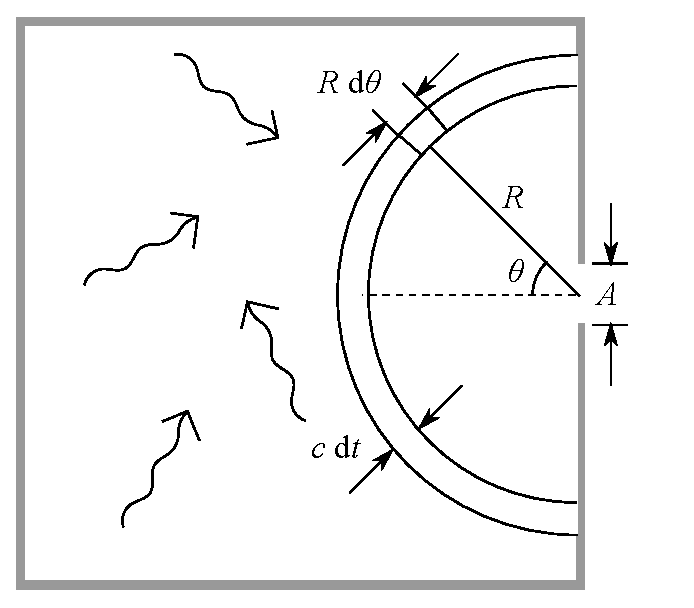
\includegraphics[height=0.3\textheight]{images/blackbody_box.eps}
\caption{\label{fig:box}{Fotonerna som lämnar lådan har en liten stund tidigare befunnit sig i samma hemisfär inne i lådan.}}
\end{figure}

Den totala mängden strålning som kommer ut kan då beräknas genom att tänka sig att de fotoner som når fram till hålet under en kort tidsperiod, $\mathrm{d}t$, alla befann sig i samma hemisfär inne i lådan för en liten stund sedan, se figur \ref{fig:box}. Tjockleken på den tänkta hemisfären är $c\mathrm{d}t$. Hemisfärens radie, $R$, beror givetvis på hur långt bak i tiden vi tittar.

Ett volymelement av hemsfären ges av
\begin{equation}
V=(R\mathrm{d}\theta) \times (R\sin\theta\mathrm{d}\phi) \times (c \mathrm{d}t).
\end{equation}

Energitäthetenför fotonerna i volymelementet är således
\begin{equation}
E_\text{v.e.}=\frac{U}{V} c \mathrm{d}t R^2 \sin\theta \mathrm{d}\theta \mathrm{d}\phi.
\end{equation}

Men endast den andel av fotonerna som har rätt riktning kommer ut genom lådans öppning. Sannoliketen för att en foton har rätt riktning är
\begin{equation}
P(\text{rätt riktning})=\frac{A\cos\theta}{4\pi R^2}
\end{equation}

där A är hålets area. Den totala energin som strålar ut ur hålet från det lilla volymselementet är alltså 
\begin{equation}
\frac{A\cos\theta}{4\pi}\frac{U}{V} c\mathrm{d}t \sin\theta\mathrm{d}\theta \mathrm{d}\phi
\end{equation}

vilket ger en total energiutstrålning på
\begin{equation}
\frac{A}{4}\frac{U}{V}c \mathrm{d}t
\end{equation}

